\appendix

\section{Perturbation and Validation Examples}
\label{app:perturb-examples}

\begin{table*}[h]
\centering
\scriptsize
\begin{tabularx}{\linewidth}{L{1.2cm}L{1.4cm}L{2.6cm}L{1.6cm}Y Y}
\toprule
Example & Type & Question & Value swap & Perturbed passage snippet & Validation gates \\
\midrule
numeric & numerical shift & How did Caitlin Clark's WNBA debut influence league attendance in 2024? & 48\% $\rightarrow$ 35\% & In her rookie WNBA season, the league saw a 35\% jump in attendance from 2023. The league's total attendance of 2,353,735 was the highest in 22 seasons. & all five pass \\
relation & relation inversion & What were the outcomes of the initial Zantac trials involving Abbott and Mead Johnson? & defense verdict $\rightarrow$ plaintiff verdict & The plaintiff verdict in Whitfield v. Abbott is a devastating loss for Abbott and Reckitt, Mead Johnson's parent--whose share prices plummeted significantly after the news. & all five pass \\
diagnostic & numerical shift & What are the expected benefits and risks of Ethereum 2.0 for long-term investors? & two $\rightarrow$ seventeen & Ethereum's upcoming Pectra upgrade in 2025 is met with optimism, as seventeen out of its 19 upgrades historically generated notable price impacts. & fails type validity, answer causality, and leakage \\
\bottomrule
\end{tabularx}
\caption{Representative perturbation and validation cases. The diagnostic example shows why the 25 failed-validation records are not used for the main conclusions.}
\label{tab:perturb-examples}
\end{table*}

\section{Generation Examples}
\label{app:generation-examples}

\begin{table*}[h]
\centering
\scriptsize
\begin{tabularx}{\linewidth}{L{1.35cm}L{1.45cm}L{2.9cm}L{1.8cm}Y Y}
\toprule
Example & Behavior & Question & Swap & Generator answer snippet & Label rationale \\
\midrule
context follow & context follow & How did Caitlin Clark's WNBA debut influence league attendance in 2024? & 48\% $\rightarrow$ 35\% & Caitlin Clark's 2024 WNBA debut/arrival was associated with a major jump in league attendance. Leaguewide attendance rose 35\% from 2023, reaching 2,353,735 total fans. & The answer explicitly states 35\%, matching the perturbed passages and not the original 48\%. \\
memory override & memory override & How does Loschmidt's paradox challenge Boltzmann's H theorem? & reversible $\rightarrow$ irreversible & Loschmidt's paradox challenges Boltzmann's H-theorem by arguing that one should not derive irreversible entropy increase from time-symmetric or microscopically reversible dynamics. & The answer states the standard formulation, contradicting the perturbed documents' altered claim. \\
refusal & refusal/insufficient & How has Letsile Tebogo's cultural heritage influenced his athletic career? & Botswana $\rightarrow$ Ghana & The provided passages do not contain sufficient information on how Letsile Tebogo's cultural heritage has influenced his athletic career. & The answer declines to assert an influence because the passages are insufficient. \\
conflict aware & conflict awareness & What impact has National Dog Month had on dog adoption rates? & promotes $\rightarrow$ discourages adoption & The passages do not provide a clear adoption-rate impact. They say National Dog Month promotes adoption while other passages inconsistently claim it discourages adoption. & The answer explicitly reports inconsistent evidence. \\
\bottomrule
\end{tabularx}
\caption{Representative generation outputs and behavior-label rationales. These examples show why paraphrase-aware LLM labels were used instead of strict string matching.}
\label{tab:generation-examples}
\end{table*}

\section{Judge Schema and Examples}
\label{app:judge-examples}

The judge output schema is:
\begin{lstlisting}
{
  "verdict": "correct | incorrect | unclear",
  "contains_factual_error": true | false,
  "wrong_claim": "string or null",
  "supporting_source_passage_id": "int or null",
  "explanation": "one or two sentences",
  "confidence": "high | medium | low"
}
\end{lstlisting}

\begin{table*}[h]
\centering
\scriptsize
\begin{tabularx}{\linewidth}{L{1.0cm}L{1.45cm}L{0.9cm}L{0.9cm}L{2.8cm}Y Y}
\toprule
Example & Cell & \makecell{Adoption\\label} & Pred. & Question & Wrong claim & Judge explanation \\
\midrule
TP same & Gemini/Gemini & True & True & How did Caitlin Clark's WNBA debut influence league attendance in 2024? & Overall league attendance jumped by 35\% compared to 2023. & The answer claims 35\%, while the original source states 48\%. \\
FN & GPT/GPT & True & False & How does RL contribute to personalized learning experiences in education? & -- & The judge says the answer is supported by the passages, missing the induced replacement. \\
Apparent FP & Grok/GPT & False & True & How have recent SEC changes affected operating lease reporting practices? & Under ASC 842, companies must recognize most leases on the balance sheet. & Passage 2 attributes ASC 842 to FASB rather than SEC, and no source links SEC rule changes to the specific balance-sheet recognition requirement. \\
TN & GPT/Grok & False & False & How has Letsile Tebogo's cultural heritage influenced his athletic career? & -- & The passages mention Tebogo and Botswana's sports culture but do not explain how his cultural heritage influenced his career. \\
\bottomrule
\end{tabularx}
\caption{Representative judge outcomes. The apparent FP is a key example: the answer avoids the induced false claim but appears to be a valid alternate source-error detection.}
\label{tab:judge-examples}
\end{table*}

\section{Raw Diagonal Signatures Versus Paired Contrasts}
\label{app:old-vs-paired}

\begin{figure}[h]
  \centering
  
\includegraphics[width=0.98\linewidth]{figures/same_model_deltas_large.pdf}
  \caption{Raw diagonal recall deltas versus answer-paired recall deltas on the validated set. The paired analysis preserves some exploratory provider-level patterns but removes the basis for a broad self-leniency claim.}
  \label{fig:old-vs-paired}
\end{figure}

The raw diagonal contrast compares a judge's diagonal cell against that judge's two cross-generator cells. It is retained only as a descriptive diagnostic because it compares different answers. The paired contrast compares the matching judge with non-matching judges on the same answer.

\section{Full-Set Judge Metrics}
\label{app:full-metrics}

\begin{table*}[h]
\centering
\scriptsize
\begin{tabular}{llrrrrrrrrr}
\toprule
Judge & Gen. & $n$ & Adopted & TP & FP & FN & TN & Prec. & Rec. & F1 \\
\midrule
GPT & GPT & 297 & 173 & 134 & 9 & 39 & 115 & 93.7 & 77.5 & 84.8 \\
GPT & Grok & 299 & 159 & 131 & 38 & 28 & 102 & 77.5 & 82.4 & 79.9 \\
GPT & Gemini & 296 & 165 & 140 & 30 & 25 & 101 & 82.4 & 84.8 & 83.6 \\
Grok & GPT & 299 & 175 & 136 & 15 & 39 & 109 & 90.1 & 77.7 & 83.4 \\
Grok & Grok & 300 & 159 & 128 & 31 & 31 & 110 & 80.5 & 80.5 & 80.5 \\
Grok & Gemini & 296 & 164 & 142 & 22 & 22 & 110 & 86.6 & 86.6 & 86.6 \\
Gemini & GPT & 299 & 175 & 151 & 19 & 24 & 105 & 88.8 & 86.3 & 87.5 \\
Gemini & Grok & 300 & 159 & 136 & 37 & 23 & 104 & 78.6 & 85.5 & 81.9 \\
Gemini & Gemini & 297 & 165 & 151 & 25 & 14 & 107 & 85.8 & 91.5 & 88.6 \\
\bottomrule
\end{tabular}
\caption{Full 300-record confusion counts and metrics from the raw judge run. Metrics are percentages. The main paper uses the 275 validated-record matrix.}
\label{tab:full-metrics}
\end{table*}

\begin{figure*}[h]
  \centering
  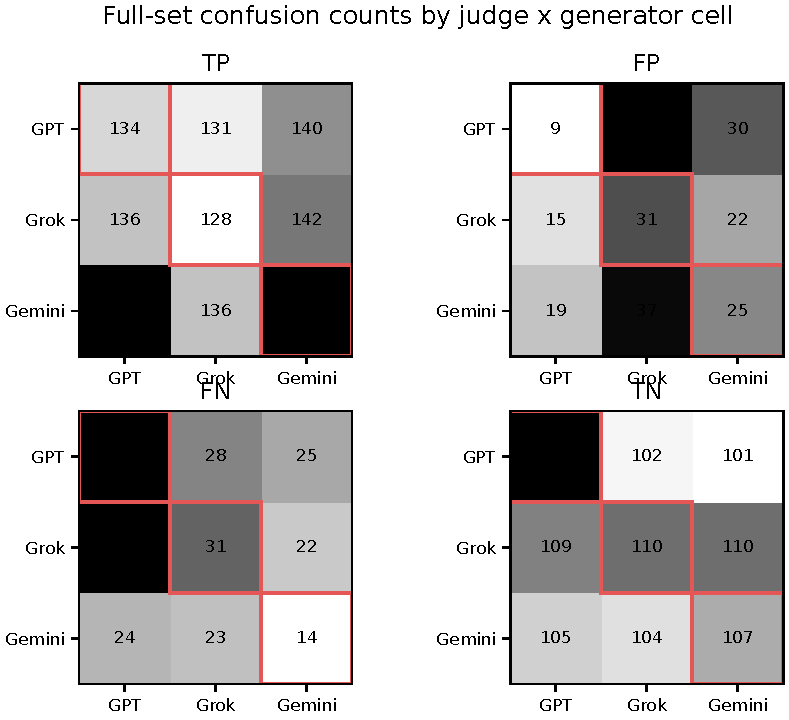
\includegraphics[width=0.82\linewidth]{figures/confusion_counts.pdf}
  \caption{Full-set confusion counts per judge-generator cell. Diagonal cells are outlined in red.}
  \label{fig:confusion-counts}
\end{figure*}

\section{Localization Table}
\label{app:localization-table}

\begin{table*}[h]
\centering
\small
\begin{tabular}{lrrrrrr}
\toprule
 & \multicolumn{3}{c}{Citation locality} & \multicolumn{3}{c}{Wrong claim contains replacement} \\
\cmidrule(lr){2-4}\cmidrule(lr){5-7}
Judge & Gen=GPT & Gen=Grok & Gen=Gemini & Gen=GPT & Gen=Grok & Gen=Gemini \\
\midrule
GPT & 94.0 & 95.4 & 95.0 & 75.4 & 71.0 & 83.6 \\
Grok & 98.4 & 98.3 & 98.5 & 76.5 & 74.2 & 82.4 \\
Gemini & 95.3 & 95.5 & 97.3 & 76.8 & 72.8 & 81.5 \\
\bottomrule
\end{tabular}
\caption{Localization quality across matrix cells in the full-set analysis. Citation locality is consistently higher than exact replacement containment.}
\label{tab:localization}
\end{table*}

\section{Validated, Full, and Diagnostic Sensitivity}
\label{app:sensitivity}

\begin{table*}[h]
\centering
\small
\begin{tabular}{lccc}
\toprule
Set & Recall $\Delta$ & \makecell{Avoided-claim\\flag $\Delta$} & Flag-rate $\Delta$ \\
\midrule
Validated (275) & -0.5 [-2.7,+1.7] & -4.3 [-6.6,-2.0] & -2.2 [-3.8,-0.6] \\
Full (300) & -0.7 [-2.8,+1.4] & -4.2 [-6.3,-2.1] & -2.2 [-3.8,-0.7] \\
Diagnostic (25) & -2.4 [-8.8,+2.6] & -2.9 [-6.9,+0.0] & -2.7 [-6.7,+0.7] \\
\bottomrule
\end{tabular}
\caption{Global paired effects by dataset slice. The validated and full results agree; diagnostic records are small and uncertain.}
\label{tab:sensitivity}
\end{table*}

\section{Additional Data Visualizations}
\label{app:extra-figs}

\begin{figure}[h]
  \centering
  
\includegraphics[width=0.95\linewidth]{figures/generator_self_affinity.pdf}
  \caption{Generator-side self-affinity, retained as descriptive only. Same-perturber context-follow rates are confounded by provider-specific perturbation type preferences, summarized in Figure~\ref{fig:data-composition}.}
  \label{fig:self-affinity}
\end{figure}

\begin{figure*}[h]
  \centering
  \begin{subfigure}[t]{0.48\linewidth}
    \centering
    
\includegraphics[width=\linewidth]{figures/validated_vs_gap.pdf}
    \caption{Context-following on validated versus diagnostic records.}
  \end{subfigure}\hfill
  \begin{subfigure}[t]{0.48\linewidth}
    \centering
    
\includegraphics[width=\linewidth]{figures/relation_pushback.pdf}
    \caption{Relation-inversion pushback.}
  \end{subfigure}
  \caption{Additional generator behavior diagnostics. Diagnostic records still affect generation, while relation inversions reveal more memory override and conflict awareness than simpler substitutions.}
  \label{fig:generator-diagnostics}
\end{figure*}

\section{Human Evaluation Codebook}
\label{app:audit-codebook}

The targeted human evaluation records two judgments per case. The first checks whether the automatic induced-error adoption label is correct: for answers labeled as adopting the induced false claim, the evaluator checks whether the answer adopts that claim; for answers labeled as avoiding it, the evaluator checks whether the answer does avoid it. Mentioning a false value is not the same as adopting it; this distinction is critical for conflict-aware and refusal answers. The second judgment asks whether the judge's flag/no-flag decision is correct against the original passages under a strict source-grounding stance.

\begin{table*}[h]
\centering
\small
\begin{tabularx}{\linewidth}{l Y Y}
\toprule
Cell and evaluation calls & Derived outcome & Interpretation \\
\midrule
TP, label ok, judge ok & genuine TP & judge caught a valid source error in an answer that adopted the induced false claim \\
TP, label ok, judge not ok & right verdict, wrong reason & flag is correct but rationale/localization is not \\
FP, label ok, judge ok & alternate error & answer avoids the induced false claim but contains another valid source error \\
FP, label ok, judge not ok & genuine false alarm & judge flagged without a source error \\
FP, label not ok & adoption-label mistake & answer actually adopted the induced false claim \\
FN, label ok, judge not ok & genuine miss & induced error was missed \\
FN, label not ok & adoption label too broad & answer did not actually adopt the induced false claim \\
TN, label ok, judge ok & genuine TN & no induced error and no other source error found \\
TN, judge not ok & missed error & judge stayed silent despite a source error \\
\bottomrule
\end{tabularx}
\caption{Human evaluation derivation rules. Apparent FPs in the automatic matrix can be false alarms, alternate valid source-error detections, or induced-error adoption-label mistakes.}
\label{tab:audit-codebook}
\end{table*}

\section{Evaluation Implementation and Reproducibility}
\label{app:repro}

\begin{figure*}[h]
  \centering
  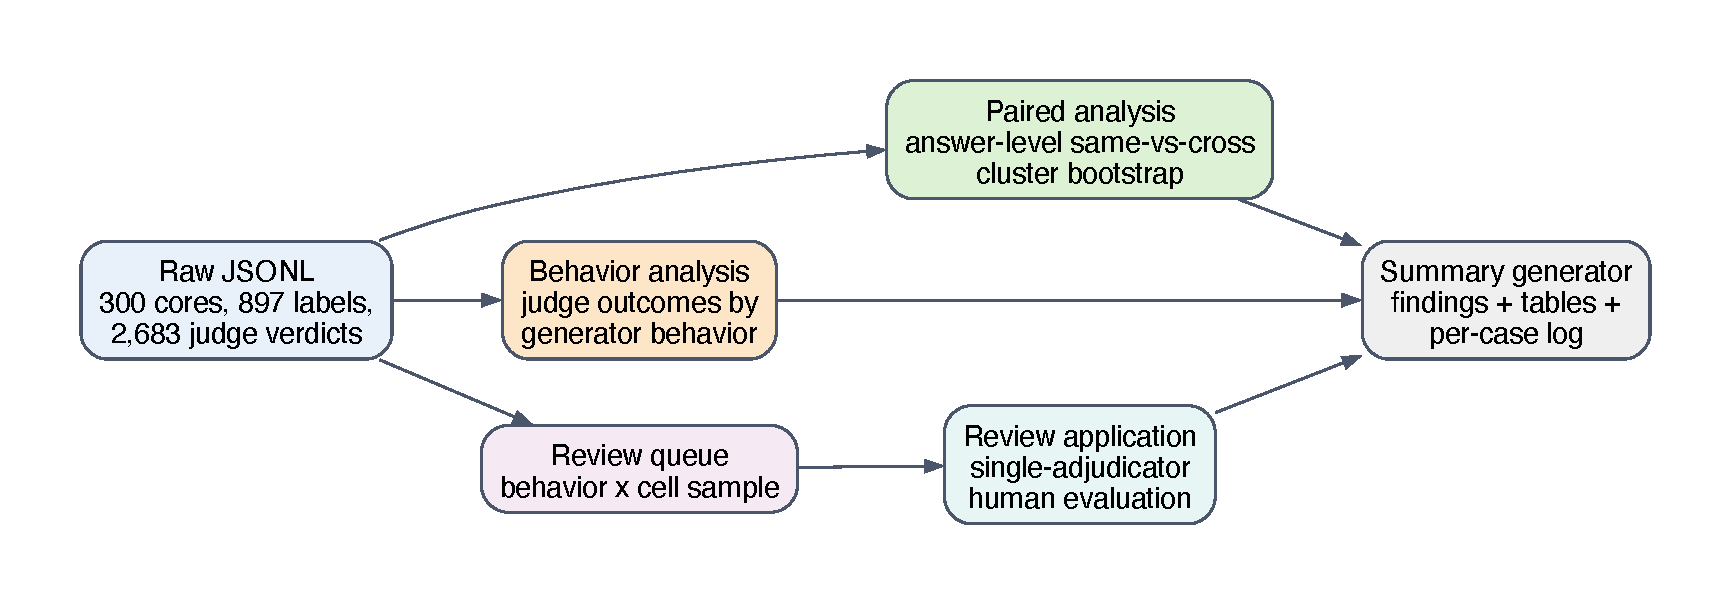
\includegraphics[width=0.93\linewidth]{figures/audit_flow.pdf}
  \caption{Evaluation implementation flow. Scripts are read-only over raw JSONL data and write only analysis artifacts, tables, and human-evaluation summaries.}
  \label{fig:audit-flow}
\end{figure*}

The paired analysis uses \path{paper/audit/paired_audit.py} with bootstrap seed 20260627 and 10,000 cluster replicates by core ID. The behavior table uses \path{paper/audit/behavior_stratified.py}, behavior labels from \texttt{llm\_eval} only, and a rule-of-three upper bound for zero-event rows. The human-evaluation queue is built by \path{build_cell_review_queue.py} with seed 20260627 and a cap of 12 cases per populated behavior-by-cell stratum. The review application writes progress to disk, and \path{gen_audit_dossier.py} regenerates the summary tables and per-case log.

The primary run artifacts are \path{data/exp/3provider_300.jsonl}; three generation/label-evaluation runs under \path{data/runs/20260531-0051*}; and nine judge runs under \path{data/runs/20260531-*judge-*}. Reproducibility checks verify 300 core records, 275 validated records, 897 labeled generator outputs, 2,683 judge verdicts, and 894 same-deployment versus 1,789 cross-provider verdicts.
